\documentclass[11pt,a4paper]{report}
\usepackage[textwidth=37em,vmargin=30mm]{geometry}
\usepackage{calc,xunicode,amsmath,amssymb,paralist,enumitem,tabu,booktabs,datetime2,xeCJK,xeCJKfntef,listings}
\usepackage{tocloft,fancyhdr,tcolorbox,xcolor,graphicx,eso-pic,xltxtra,xelatexemoji}

\newcommand{\envyear}[0]{2025}
\newcommand{\envdatestr}[0]{2025-03-22}
\newcommand{\envfinaldir}[0]{webdb/2025/20250322/final}

\usepackage[hidelinks]{hyperref}
\hypersetup{
    colorlinks=false,
    pdfpagemode=FullScreen,
    pdftitle={Web Digest - \envdatestr}
}

\setlength{\cftbeforechapskip}{10pt}
\renewcommand{\cftchapfont}{\rmfamily\bfseries\large\raggedright}
\setlength{\cftbeforesecskip}{2pt}
\renewcommand{\cftsecfont}{\sffamily\small\raggedright}

\setdefaultleftmargin{2em}{2em}{1em}{1em}{1em}{1em}

\usepackage{xeCJK,xeCJKfntef}
\xeCJKsetup{PunctStyle=plain,RubberPunctSkip=false,CJKglue=\strut\hskip 0pt plus 0.1em minus 0.05em,CJKecglue=\strut\hskip 0.22em plus 0.2em}
\XeTeXlinebreaklocale "zh"
\XeTeXlinebreakskip = 0pt


\setmainfont{Brygada 1918}
\setromanfont{Brygada 1918}
\setsansfont{IBM Plex Sans}
\setmonofont{JetBrains Mono NL}
\setCJKmainfont{Noto Serif CJK SC}
\setCJKromanfont{Noto Serif CJK SC}
\setCJKsansfont{Noto Sans CJK SC}
\setCJKmonofont{Noto Sans CJK SC}

\setlength{\parindent}{0pt}
\setlength{\parskip}{8pt}
\linespread{1.15}

\lstset{
	basicstyle=\ttfamily\footnotesize,
	numbersep=5pt,
	backgroundcolor=\color{black!5},
	showspaces=false,
	showstringspaces=false,
	showtabs=false,
	tabsize=2,
	captionpos=b,
	breaklines=true,
	breakatwhitespace=true,
	breakautoindent=true,
	linewidth=\textwidth
}






\newcommand{\coverpic}[2]{
    % argv: itemurl, authorname
    Cover photo by #2~~(\href{#1}{#1})
}
\newcommand{\makeheader}[0]{
    \begin{titlepage}
        % \newgeometry{hmargin=15mm,tmargin=21mm,bmargin=12mm}
        \begin{center}
            
            \rmfamily\scshape
            \fontspec{BaskervilleF}
            \fontspec{Old Standard}
            \fontsize{59pt}{70pt}\selectfont
            WEB\hfill DIGEST
            
            \vfill
            % \vskip 30pt
            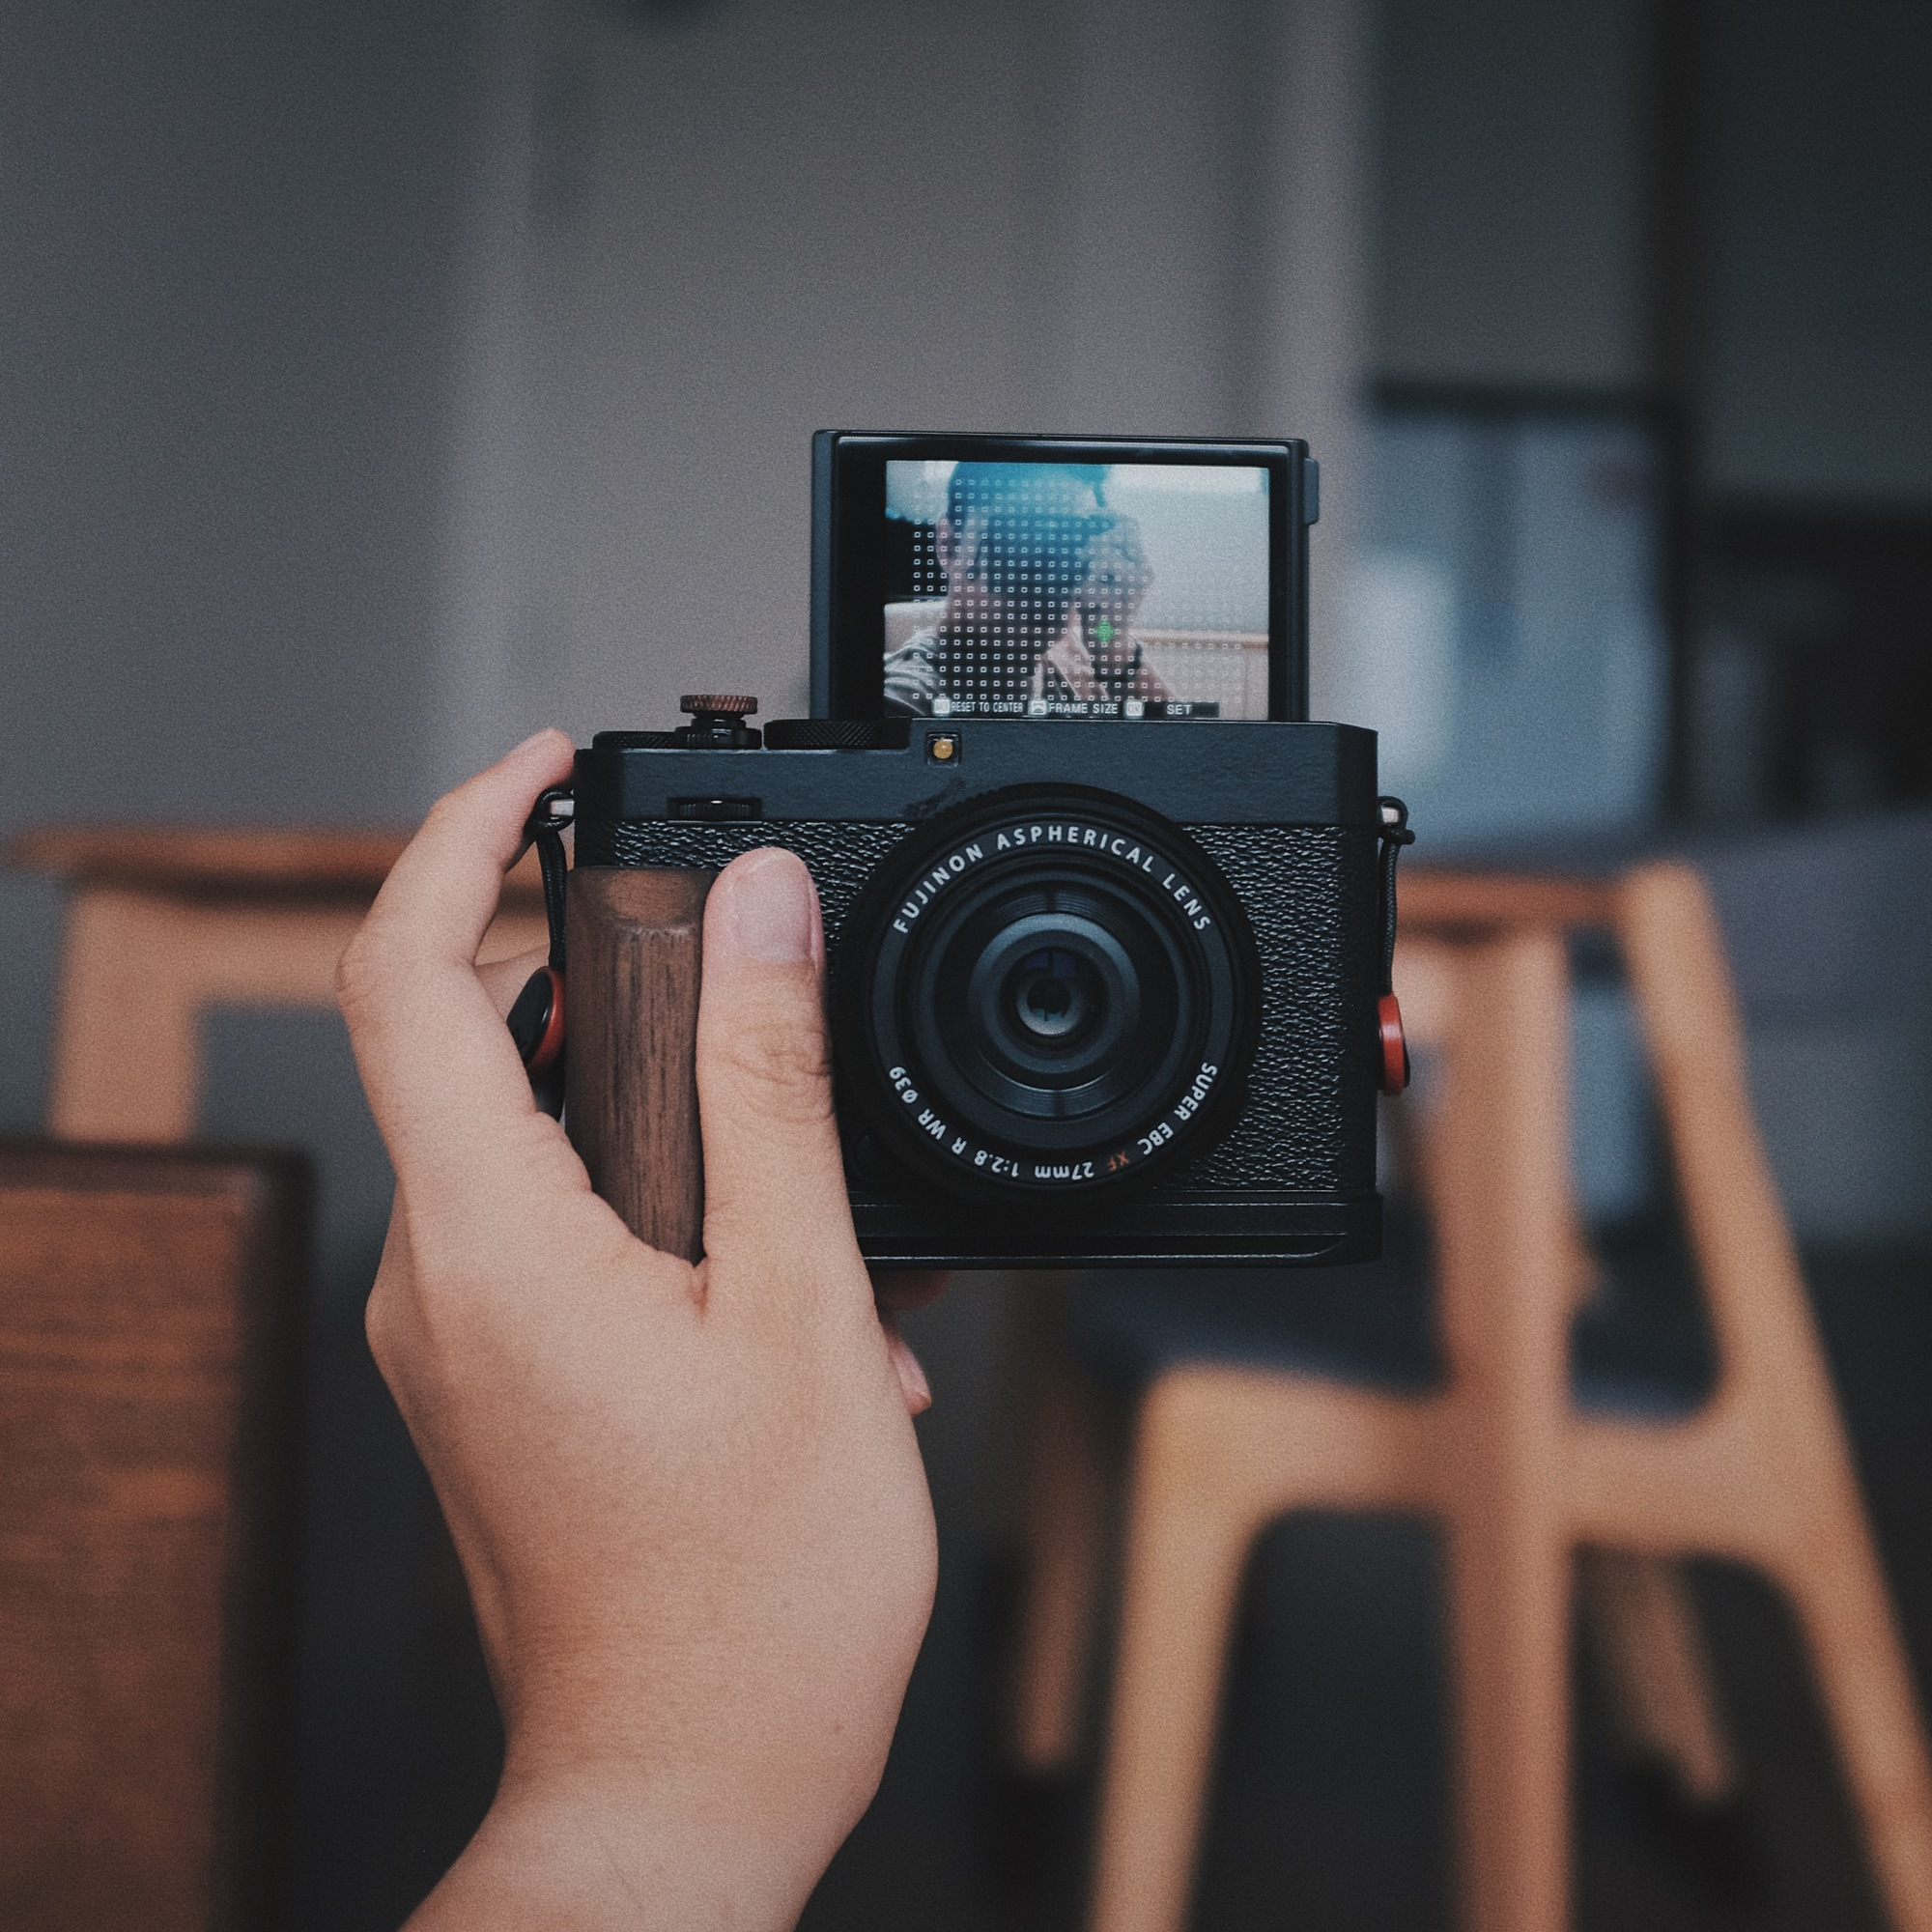
\includegraphics[width=\linewidth]{\envfinaldir/coverpic-prod.jpg}\par
            % \vskip 30pt
            \vfill

            \normalsize\rmfamily\scshape
            \copyright{} The Web Digest Project \hfill\large \envdatestr
        \end{center}
    \end{titlepage}
    % \restoregeometry
}
\newcommand{\simplehref}[1]{%
    \textcolor{blue!80!green}{\href{#1}{#1}}%
}
\renewcommand{\contentsname}{\center\Huge\sffamily\bfseries Contents\par\vskip 20pt}
\newcounter{ipartcounter}
\setcounter{ipartcounter}{0}
\newcommand{\ipart}[1]{
    % \vskip 20pt
    \clearpage
    \stepcounter{ipartcounter}
    \phantomsection
    \addcontentsline{toc}{chapter}{#1}
    % \begin{center}
    %     \Huge
    %     \sffamily\bfseries
    %     #1
    % \end{center}
    % \vskip 20pt plus 7pt
}
\newcounter{ichaptercounter}
\setcounter{ichaptercounter}{0}
\newcommand{\ichapter}[1]{
    % \vskip 20pt
    \clearpage
    \stepcounter{ichaptercounter}
    \phantomsection
    \addcontentsline{toc}{section}{\numberline{\arabic{ichaptercounter}}#1}
    \begin{center}
        \Huge
        \sffamily\bfseries
        #1
    \end{center}
    \vskip 20pt plus 7pt
}
\newcommand{\entrytitlefont}[1]{\subsection*{\raggedright\Large\sffamily\bfseries#1}}
\newcommand{\entryitemGeneric}[2]{
    % argv: title, url
    \parbox{\linewidth}{
        \entrytitlefont{#1}\par\vskip 5pt
        \footnotesize\ttfamily\mdseries
        \simplehref{#2}
    }\vskip 11pt plus 11pt minus 1pt
}
\newcommand{\entryitemGithub}[3]{
    % argv: title, url, desc
    \parbox{\linewidth}{
        \entrytitlefont{#1}\par\vskip 5pt
        \footnotesize\ttfamily\mdseries
        \simplehref{#2}\par\vskip 5pt
        \small\rmfamily\mdseries#3
    }\vskip 11pt plus 11pt minus 1pt
}
\newcommand{\entryitemAp}[3]{
    % argv: title, url, desc
    \parbox{\linewidth}{
        \entrytitlefont{#1}\par\vskip 5pt
        \footnotesize\ttfamily\mdseries
        \simplehref{#2}\par\vskip 5pt
        \small\rmfamily\mdseries#3
    }\vskip 11pt plus 11pt minus 1pt
}
\newcommand{\entryitemHackernews}[3]{
    % argv: title, hnurl, rawurl
    % \parbox{\linewidth}{
    %     \entrytitlefont{#1}\par\vskip 5pt
    %     \footnotesize\ttfamily\mdseries
    %     \simplehref{#3}\par
    %     \textcolor{black!50}{\href{#2}{#2}}
    % }\vskip 11pt plus 11pt minus 1pt
    \begin{minipage}{\linewidth}
            \entrytitlefont{#1}\par\vskip 5pt
            \footnotesize\ttfamily\mdseries
            \simplehref{#3}\par
            \textcolor{black!50}{\href{#2}{#2}}
    \end{minipage}\par\vskip 11pt plus 11pt minus 1pt
}







\begin{document}

\makeheader

\tableofcontents\clearpage




\ipart{Developers}
\ichapter{Hacker News}
\entryitemTwoLinks{France rejects backdoor mandate}{https://news.ycombinator.com/item?id=43440513}{https://www.eff.org/deeplinks/2025/03/win-encryption-france-rejects-backdoor-mandate}

\entryitemTwoLinks{The little book about OS development}{https://news.ycombinator.com/item?id=43440473}{https://littleosbook.github.io/}

\entryitemTwoLinks{Pen and Paper Exercises in Machine Learning (2022)}{https://news.ycombinator.com/item?id=43440267}{https://arxiv.org/abs/2206.13446}

\entryitemTwoLinks{New USPTO Memo Makes Fighting Patent Trolls Even Harder}{https://news.ycombinator.com/item?id=43439610}{https://www.eff.org/deeplinks/2025/03/new-uspto-memo-makes-fighting-patent-trolls-even-harder}

\entryitemTwoLinks{Show HN: A terminal emulator in pure PHP}{https://news.ycombinator.com/item?id=43438797}{https://github.com/soloterm/screen}

\entryitemTwoLinks{Bigscreen Beyond 2}{https://news.ycombinator.com/item?id=43438206}{https://www.bigscreenvr.com/}

\entryitemTwoLinks{IronRDP: a Rust implementation of Microsoft's RDP protocol}{https://news.ycombinator.com/item?id=43436894}{https://github.com/Devolutions/IronRDP}

\entryitemTwoLinks{The Road Not Taken Is Guaranteed Minimum Income}{https://news.ycombinator.com/item?id=43436454}{https://blog.codinghorror.com/the-road-not-taken-is-guaranteed-minimum-income/}

\entryitemTwoLinks{Congestion Pricing Is a Policy Miracle}{https://news.ycombinator.com/item?id=43436315}{https://bettercities.substack.com/p/congestion-pricing-is-a-policy-miracle}

\entryitemTwoLinks{Show HN: Torch Lens Maker – Differentiable Geometric Optics in PyTorch}{https://news.ycombinator.com/item?id=43435438}{https://victorpoughon.github.io/torchlensmaker/}

\entryitemTwoLinks{Wheel Reinventor's Principles (2024)}{https://news.ycombinator.com/item?id=43434730}{https://tobloef.com/blog/wheel-reinventors-principles/}

\entryitemTwoLinks{Imagine telling 2010 devs that in 2025, collapsing a div would require \$8/ month}{https://news.ycombinator.com/item?id=43434466}{https://old.reddit.com/r/webdev/comments/1jged6g/imagine\_telling\_2010\_devs\_that\_in\_2025\_collapsing/}

\entryitemTwoLinks{Notetime: Minimalistic notes where everything is timestamped}{https://news.ycombinator.com/item?id=43434152}{https://www.notetimeapp.com}

\entryitemTwoLinks{Career Development: What It Means to Be a Manager, Director, or VP (2015)}{https://news.ycombinator.com/item?id=43434093}{https://kellblog.com/2015/03/08/career-development-what-it-really-means-to-be-a-manager-director-or-vp/}

\entryitemTwoLinks{The FBI Seized This Woman's Life Savings–Without Telling Her Why}{https://news.ycombinator.com/item?id=43433694}{https://reason.com/2025/03/20/the-fbi-seized-this-womans-life-savings-without-telling-her-why/}

\entryitemTwoLinks{Germany tightens travel advice to US after three citizens detained}{https://news.ycombinator.com/item?id=43433071}{https://www.euronews.com/my-europe/2025/03/19/germany-tightens-travel-advice-to-us-after-three-citizens-detained}

\entryitemTwoLinks{Calibre 8.0}{https://news.ycombinator.com/item?id=43432890}{https://calibre-ebook.com/whats-new}

\entryitemTwoLinks{Boycott IETF 127}{https://news.ycombinator.com/item?id=43431780}{https://boycott-ietf127.org/}

\entryitemTwoLinks{Apple shuffles AI executive ranks in bid to turn around Siri}{https://news.ycombinator.com/item?id=43431675}{https://finance.yahoo.com/news/apple-shuffles-ai-executive-ranks-162500488.html}

\entryitemTwoLinks{London's Heathrow Airport announces complete shutdown due to power outage}{https://news.ycombinator.com/item?id=43431567}{https://www.cnn.com/2025/03/20/travel/london-heathrow-airport-shut-intl-hnk/index.html}\ichapter{Phoronix}
\entryitemGeneric{\hskip 0pt{}Wine 10.4 Brings More Direct3D To Vulkan Video Handling, Continued Bluetooth Driver Work}{https://www.phoronix.com/news/Wine-10.4-Released}

\entryitemGeneric{\hskip 0pt{}AMD Announces AITER For ROCm To Help Boost AI Performance}{https://www.phoronix.com/news/AMD-AITER-AI-Performance-ROCm}

\entryitemGeneric{\hskip 0pt{}Microsoft Proposes "Hornet" Security Module For The Linux Kernel}{https://www.phoronix.com/news/Microsoft-Hornet-Linux-LSM}

\entryitemGeneric{\hskip 0pt{}ReactOS 0.4.15 Released For This "Open-Source Windows" OS With Tons Of Enhancements}{https://www.phoronix.com/news/ReactOS-0.4.15-Released}

\entryitemGeneric{\hskip 0pt{}Linux Security Hardening Cache Randomization Was Inadvertently Using The Same Seed}{https://www.phoronix.com/news/Linux-6.15-slab}

\entryitemGeneric{\hskip 0pt{}New Intel/AMD GPU Features, Apple Touch Bar Drivers \& Other Likely Changes For Linux 6.15}{https://www.phoronix.com/news/Linux-6.15-Likely-Features}

\entryitemGeneric{\hskip 0pt{}Raspberry Pi Announces rpi-image-gen To Help Craft Custom Software Images}{https://www.phoronix.com/news/Raspberry-Pi-rpi-image-gen}

\entryitemGeneric{\hskip 0pt{}Linux 6.14 Sees Last Minute Fix For A Two Year Old Regression Causing A 30\% Performance Drop}{https://www.phoronix.com/news/Linux-6.14-Sched-2-Year-Regress}

\entryitemGeneric{\hskip 0pt{}AMD Announces Open-Source "GAIA" For GenAI But Currently Windows-Only}{https://www.phoronix.com/news/AMD-GAIA-Open-Source}\ichapter{Dribbble}
\entryitemGeneric{\hskip 0pt{}PurePaws - Logo Design}{https://dribbble.com/shots/25797575-PurePaws-Logo-Design}

\entryitemGeneric{\hskip 0pt{}S mark}{https://dribbble.com/shots/25796446-S-mark}

\entryitemGeneric{\hskip 0pt{}Central Coast}{https://dribbble.com/shots/25794367-Central-Coast}

\entryitemGeneric{\hskip 0pt{}The Sequencer Poster}{https://dribbble.com/shots/25798231-The-Sequencer-Poster}

\entryitemGeneric{\hskip 0pt{}Puzzle Fintech UI/UX design, User Interface experience}{https://dribbble.com/shots/25652036-Puzzle-Fintech-UI-UX-design-User-Interface-experience}

\entryitemGeneric{\hskip 0pt{}Novascan}{https://dribbble.com/shots/25790443-Novascan}

\entryitemGeneric{\hskip 0pt{}Sidebar Navigation for Core 2.0 – Dashboard Builder}{https://dribbble.com/shots/25790810-Sidebar-Navigation-for-Core-2-0-Dashboard-Builder}

\entryitemGeneric{\hskip 0pt{}Plain - Branding}{https://dribbble.com/shots/25790107-Plain-Branding}

\entryitemGeneric{\hskip 0pt{}Halo Movie poster}{https://dribbble.com/shots/25791667-Halo-Movie-poster}

\entryitemGeneric{\hskip 0pt{}Crypto Bridge}{https://dribbble.com/shots/25783744-Crypto-Bridge}

\entryitemGeneric{\hskip 0pt{}Eclipse - Logo Design}{https://dribbble.com/shots/25784396-Eclipse-Logo-Design}

\entryitemGeneric{\hskip 0pt{}Cargo Shipment App UI}{https://dribbble.com/shots/25784159-Cargo-Shipment-App-UI}

\entryitemGeneric{\hskip 0pt{}Burn Bright, Take Flight}{https://dribbble.com/shots/25778930-Burn-Bright-Take-Flight}

\entryitemGeneric{\hskip 0pt{}The Planner app}{https://dribbble.com/shots/25769751-The-Planner-app}

\entryitemGeneric{\hskip 0pt{}PieLabs Unused Logo Design}{https://dribbble.com/shots/25784372-PieLabs-Unused-Logo-Design}

\entryitemGeneric{\hskip 0pt{}Rose Logo Design [for sale]}{https://dribbble.com/shots/25775027-Rose-Logo-Design-for-sale}

\entryitemGeneric{\hskip 0pt{}Mammut Logo Redesign Concept}{https://dribbble.com/shots/25776663-Mammut-Logo-Redesign-Concept}

\entryitemGeneric{\hskip 0pt{}Cimet Logo Grid}{https://dribbble.com/shots/25710567-Cimet-Logo-Grid}

\entryitemGeneric{\hskip 0pt{}Bento grid \& dashboard for revops startup}{https://dribbble.com/shots/25765472-Bento-grid-dashboard-for-revops-startup}

\entryitemGeneric{\hskip 0pt{}Glide wallet}{https://dribbble.com/shots/25768771-Glide-wallet}

\entryitemGeneric{\hskip 0pt{}DL}{https://dribbble.com/shots/25775198-DL}

\entryitemGeneric{\hskip 0pt{}bigbeardamian: Badge Design}{https://dribbble.com/shots/25737398-bigbeardamian-Badge-Design}

\entryitemGeneric{\hskip 0pt{}Fitme}{https://dribbble.com/shots/25766813-Fitme}

\entryitemGeneric{\hskip 0pt{}Illustration}{https://dribbble.com/shots/25767159-Illustration}


\ipart{Developers~~~~(zh-Hans)}
\ichapter{Solidot}
\entryitemGeneric{\hskip 0pt{}Calibre 8.0 释出}{https://www.solidot.org/story?sid=80848}

\entryitemGeneric{\hskip 0pt{}Gmail 引入 AI 驱动的搜索}{https://www.solidot.org/story?sid=80847}

\entryitemGeneric{\hskip 0pt{}英伟达在 GTC 会议期间用流动餐车卖 2000 张显卡}{https://www.solidot.org/story?sid=80846}

\entryitemGeneric{\hskip 0pt{}海豹能感知其血液中的氧含量而避免溺水}{https://www.solidot.org/story?sid=80845}

\entryitemGeneric{\hskip 0pt{}自由开源软件基础设施面临来自 AI 公司的攻击}{https://www.solidot.org/story?sid=80844}

\entryitemGeneric{\hskip 0pt{}婴儿能编码短暂的海马体记忆 }{https://www.solidot.org/story?sid=80843}

\entryitemGeneric{\hskip 0pt{}2023/24 年海洋表面温度大幅上升}{https://www.solidot.org/story?sid=80842}

\entryitemGeneric{\hskip 0pt{}GNOME 48 释出}{https://www.solidot.org/story?sid=80841}

\entryitemGeneric{\hskip 0pt{}Euclid 探测器公布首批观测结果}{https://www.solidot.org/story?sid=80840}

\entryitemGeneric{\hskip 0pt{}转基因细菌能生产出塑料}{https://www.solidot.org/story?sid=80839}

\entryitemGeneric{\hskip 0pt{}尼安德特人可能吃蛆虫}{https://www.solidot.org/story?sid=80838}

\entryitemGeneric{\hskip 0pt{}微塑料会增强大肠杆菌的耐药性}{https://www.solidot.org/story?sid=80837}

\entryitemGeneric{\hskip 0pt{}土耳其逮捕反对派领导人限制互联网}{https://www.solidot.org/story?sid=80836}

\entryitemGeneric{\hskip 0pt{}软银以 65 亿美元收购芯片设计公司 Ampere}{https://www.solidot.org/story?sid=80835}

\entryitemGeneric{\hskip 0pt{}鹦鹉如何模仿人类说话}{https://www.solidot.org/story?sid=80834}

\entryitemGeneric{\hskip 0pt{}PCI Express 7 即将完成,但 PCI Express 6 尚无普及}{https://www.solidot.org/story?sid=80833}

\entryitemGeneric{\hskip 0pt{}欧盟要求苹果开放生态系统否则将面临罚款}{https://www.solidot.org/story?sid=80832}

\entryitemGeneric{\hskip 0pt{}百度否认开盒信息来自该公司}{https://www.solidot.org/story?sid=80831}

\entryitemGeneric{\hskip 0pt{}Gemini 2.0 Flash 让任何人都能 PS}{https://www.solidot.org/story?sid=80830}

\entryitemGeneric{\hskip 0pt{}PC 玩家 92\% 的时间是在老游戏上}{https://www.solidot.org/story?sid=80829}\ichapter{V2EX}
\entryitemGeneric{\hskip 0pt{}[iOS] iOS 上有没有媲美 Linearity Curve 的 app?}{https://www.v2ex.com/t/1120253}

\entryitemGeneric{\hskip 0pt{}[问与答] 一个客户端 Android(/iOS)开发 利用 cursor/openai 如何做服务端开发,例如接口开发,数据管理,不用考虑高并发情况}{https://www.v2ex.com/t/1120252}

\entryitemGeneric{\hskip 0pt{}[问与答] 真机与逆向有什么区别}{https://www.v2ex.com/t/1120251}

\entryitemGeneric{\hskip 0pt{}[Chrome] 四个能增强 Edge 安全感的插件}{https://www.v2ex.com/t/1120250}

\entryitemGeneric{\hskip 0pt{}[职场话题] 今天一句话让我体验到国内外文化差异}{https://www.v2ex.com/t/1120249}

\entryitemGeneric{\hskip 0pt{}[macOS] highlights app 标记 pdf 很好用,奈何不喜欢订阅制,请问有什么办法可以买断或者开心版?}{https://www.v2ex.com/t/1120248}

\entryitemGeneric{\hskip 0pt{}[问与答] 手上有些钱,想创业往 AI 方向发展,能给点建议吗?}{https://www.v2ex.com/t/1120247}

\entryitemGeneric{\hskip 0pt{}[宽带症候群] 专业技术贴 关于交换机与猫棒}{https://www.v2ex.com/t/1120246}

\entryitemGeneric{\hskip 0pt{}[程序员] 鹅厂前同事下海经商,正在倒腾一个相亲小程序[无广告]}{https://www.v2ex.com/t/1120245}

\entryitemGeneric{\hskip 0pt{}[Go 编程语言] 今天有个面试官和我讲 go 的协程比系统的线程更慢,这个我不能理解}{https://www.v2ex.com/t/1120244}

\entryitemGeneric{\hskip 0pt{}[VPS] 请问付了一年前斯巴达的服务工单还能正常用吗,和搬瓦工 Plan 比该留哪一个}{https://www.v2ex.com/t/1120242}

\entryitemGeneric{\hskip 0pt{}[问与答] 好像没有老年人友好型的滚筒洗衣机/烘干机?}{https://www.v2ex.com/t/1120241}

\entryitemGeneric{\hskip 0pt{}[VPS] 一图读懂搬瓦工 DC99 机房 Biggerbox 升级路径}{https://www.v2ex.com/t/1120240}

\entryitemGeneric{\hskip 0pt{}[Apple] apple music 港区搭个车}{https://www.v2ex.com/t/1120239}

\entryitemGeneric{\hskip 0pt{}[程序员] C++ 开发不想 996,如何跳槽转到 Java ?}{https://www.v2ex.com/t/1120238}

\entryitemGeneric{\hskip 0pt{}[生活] 过去了 60 天了,我的副业照片打印是否还能继续?}{https://www.v2ex.com/t/1120237}

\entryitemGeneric{\hskip 0pt{}[NAS] 如何把硬飞牛迁移到 PVE 中去?}{https://www.v2ex.com/t/1120236}

\entryitemGeneric{\hskip 0pt{}[职场话题] 18 毕业直到现在都是在北京干桌面运维,下个月离职,有必要去上海找工作继续干桌面运维吗}{https://www.v2ex.com/t/1120233}

\entryitemGeneric{\hskip 0pt{}[问与答] Typescript 如此成功,为何没有发展出所谓 ``Typthon''?}{https://www.v2ex.com/t/1120232}

\entryitemGeneric{\hskip 0pt{}[macOS] mbp 选购决赛圈,大佬们,快快快!}{https://www.v2ex.com/t/1120231}

\entryitemGeneric{\hskip 0pt{}[职场话题] 有人了解小熊博望这家公司吗?}{https://www.v2ex.com/t/1120229}

\entryitemGeneric{\hskip 0pt{}[职场话题] 求助 v 友,你们可以作一下经验之谈吗}{https://www.v2ex.com/t/1120226}

\entryitemGeneric{\hskip 0pt{}[问与答] go 语言值得学一学吗?未来前景怎么样}{https://www.v2ex.com/t/1120225}

\entryitemGeneric{\hskip 0pt{}[Apple] 切换到外区后, icloud 同步异常}{https://www.v2ex.com/t/1120224}

\entryitemGeneric{\hskip 0pt{}[分享发现] Draw.io:你可能不知道的「白嫖级」图表绘制神器}{https://www.v2ex.com/t/1120222}

\entryitemGeneric{\hskip 0pt{}[分享发现] 数字身份分割术:现代隐私防护体系构建防开盒操作指南}{https://www.v2ex.com/t/1120221}

\entryitemGeneric{\hskip 0pt{}[问与答] Windows 上有没有软件白名单功能的代理软件?}{https://www.v2ex.com/t/1120220}

\entryitemGeneric{\hskip 0pt{}[职场话题] AI 时代,高并发经历对于职业是否必须?}{https://www.v2ex.com/t/1120219}

\entryitemGeneric{\hskip 0pt{}[程序员] 大家都是怎么获得那些前沿的 ai(应用)的信息}{https://www.v2ex.com/t/1120217}

\entryitemGeneric{\hskip 0pt{}[宽带症候群] 坐标 0738,被标记大流量,掐了 IPv6,上行限死 2Mbps}{https://www.v2ex.com/t/1120216}

\entryitemGeneric{\hskip 0pt{}[问与答] ios 浏览器能否实现点击图片下载?}{https://www.v2ex.com/t/1120215}

\entryitemGeneric{\hskip 0pt{}[问与答] 一个纯后端人员可以依靠 cursor/trae/其他的 aiide 实现一个 app 吗,只需要有简单功能就行的那种(哪怕只是实现一个加减乘除的计算器)}{https://www.v2ex.com/t/1120214}

\entryitemGeneric{\hskip 0pt{}[问与答] OLED 手机与结膜炎}{https://www.v2ex.com/t/1120213}

\entryitemGeneric{\hskip 0pt{}[推广] [网站自荐] ​一个用来筛选大流量电话卡的 AI 导购员}{https://www.v2ex.com/t/1120212}

\entryitemGeneric{\hskip 0pt{}[问与答] 入手了国补教育优惠 ipadair 有什么游戏推荐吗}{https://www.v2ex.com/t/1120211}

\entryitemGeneric{\hskip 0pt{}[Android] 推荐个安卓手机}{https://www.v2ex.com/t/1120210}

\entryitemGeneric{\hskip 0pt{}[深圳] 51 去云南旅行注意事项}{https://www.v2ex.com/t/1120208}

\entryitemGeneric{\hskip 0pt{}[酷工作] [深圳] iOS 开发工程师, 20k-23k}{https://www.v2ex.com/t/1120207}

\entryitemGeneric{\hskip 0pt{}[Go 编程语言] 朋友们,有哪些基于 Gin 框架的优秀开源项目,用来学习?}{https://www.v2ex.com/t/1120205}

\entryitemGeneric{\hskip 0pt{}[程序员] https://www.openai.fm/ 今天的乐子}{https://www.v2ex.com/t/1120204}

\entryitemGeneric{\hskip 0pt{}[分享发现] 蜗居赚钱}{https://www.v2ex.com/t/1120203}

\entryitemGeneric{\hskip 0pt{}[问与答] 需求:如何用 llm 大规模翻译英文文档}{https://www.v2ex.com/t/1120202}

\entryitemGeneric{\hskip 0pt{}[Apple] 切肤之痛,奉劝各位有出差需求但是又想扩容的慎重}{https://www.v2ex.com/t/1120201}

\entryitemGeneric{\hskip 0pt{}[程序员] github 被 Suspended 后账号会永久删除吗}{https://www.v2ex.com/t/1120200}

\entryitemGeneric{\hskip 0pt{}[iPhone] 拼多多上买 iphone16pro 256G 靠谱吗?}{https://www.v2ex.com/t/1120199}

\entryitemGeneric{\hskip 0pt{}[酷工作] [深圳线下] 招聘后端, 15k-22k,小而美公司,快来快来!}{https://www.v2ex.com/t/1120198}

\entryitemGeneric{\hskip 0pt{}[分享发现] 微软真是有大病,自家的软件不给 win 用}{https://www.v2ex.com/t/1120197}

\entryitemGeneric{\hskip 0pt{}[问与答] 香港汇丰开户超级快啊}{https://www.v2ex.com/t/1120196}

\entryitemGeneric{\hskip 0pt{}[分享创造] [chrome 插件] IT 之家阅读体验增强器: IThome Purer}{https://www.v2ex.com/t/1120195}

\entryitemGeneric{\hskip 0pt{}[生活] 有没有走过交通事故行政复议的兄弟,我这种情况有必要复议或诉讼吗?}{https://www.v2ex.com/t/1120194}


\ipart{Generic News}







\clearpage
\leavevmode\vfill
\footnotesize

Copyright \copyright{} 2023-2025 Neruthes and other contributors.

This document is published with CC BY-NC-ND 4.0 license.

The entries listed in this newsletter may be copyrighted by their respective creators.

This newsletter is generated by the Web Digest project.

The newsletters are also delivered via Telegram channel \CJKunderline{\href{https://t.me/webdigestchannel}{https://t.me/webdigestchannel}}.\\
RSS feed is available at \CJKunderline{\href{https://webdigest.pages.dev/rss.xml}{https://webdigest.pages.dev/rss.xml}}.

This newsletter is available in PDF at
\CJKunderline{\href{https://webdigest.pages.dev/}{https://webdigest.pages.dev/}}.

The source code being used to generate this newsletter is available at\\
\CJKunderline{\href{https://github.com/neruthes/webdigest}{https://github.com/neruthes/webdigest}}.

This newsletter is also available in
\CJKunderline{\href{http://webdigest.pages.dev/readhtml/\envyear/WebDigest-20250322.html}{HTML}} and
\CJKunderline{\href{https://github.com/neruthes/webdigest/blob/master/markdown/\envyear/WebDigest-20250322.md}{Markdown}}.


\coverpic{https://unsplash.com/photos/people-are-skiing-on-a-snowy-mountain-iBAKOYi-vVQ}{LOGAN WEAVER | @LGNWVR}


\end{document}
